% --------------------------------------------------------------------
% LaTeX Template for Math Homework
% --------------------------------------------------------------------

\documentclass{article}

% --- PACKAGE IMPORTS ---
% These packages add functionality for math symbols, formatting, etc.
\usepackage[margin=.7in]{geometry}       % For setting page margins
\usepackage{amsmath, amssymb, amsthm}   % American Mathematical Society packages for advanced math
\usepackage{graphicx}                   % For including images
\usepackage{fancyhdr}                   % For creating custom headers and footers
\usepackage[colorlinks=true, urlcolor=blue, linkcolor=blue]{hyperref} % For clickable links
\usepackage{cancel}
\usepackage{array}
\usepackage{amsfonts}
\usepackage{amsxtra}
\usepackage{epsfig}
\usepackage{wasysym}
\usepackage{relsize}
\usepackage{tikz}
\tikzset{every picture/.style={scale=1.2}}
\usetikzlibrary{decorations.markings} 
\renewcommand{\normalsize}{\fontsize{12}{20}\selectfont}

% custom commands
\newcommand{\myauthor}{Miguel Gomez}
\newcommand{\canceling}[2]{\textcolor{red}{\cancelto{\textcolor{black}{#1}}{\textcolor{black}{#2}}}}
\newcommand{\todo}[1]{\textcolor{blue}{TODO:#1}}
% Save the original commands
\let\oldcos\cos
\let\oldsin\sin
\let\oldcosh\cosh
\let\oldsinh\sinh

% Redefine with automatic parentheses
\renewcommand{\cos}[1]{\oldcos\left(#1\right)}
\renewcommand{\sin}[1]{\oldsin\left(#1\right)}
\renewcommand{\cosh}[1]{\oldcosh\left(#1\right)}
\renewcommand{\sinh}[1]{\oldsinh\left(#1\right)}

\newcommand{\der}[2]{\frac{d#1}{d#2}}
\newcommand{\secder}[2]{\frac{d^2#1}{d#2^2}}
\newcommand{\parder}[2]{\frac{\partial#1}{\partial#2}}
\newcommand{\secparder}[2]{\frac{\partial^2#1}{\partial#2^2}}

% --- DOCUMENT & AUTHOR INFORMATION ---
\title{Homework \# 6}
\author{
  MATH 3160 -- Complex Variables\\
  \myauthor
}
\date{Completed: \today}

% --- HEADER & FOOTER CONFIGURATION ---
% This section sets up the header that will appear on each page.
\pagestyle{fancy}
\fancyhf{} % Clears the default header and footer
\lhead{Math 3160 -- HW \# 6} % Left side of header
\rhead{\myauthor} % Puts the author's name on the right side
\rfoot{Page \thepage} % Puts the page number on the bottom right

\begin{document}

\maketitle % This command generates the title based on the information above.

% ====================================================================
% --- START OF PROBLEMS ---
% ====================================================================

\section*{Problem 1}
Find parameterized representations $z(t)$ of the following contours in the plane including $t$-ranges.
\begin{enumerate}
\item  A straight line from point $(1+2i)$ to point $(i+2)$
\item A line from $(0,0)$ to point $(1+\sqrt{3}i)$
\item A half-ellipse from point $2$ to $-2$ passing through $i$ centered at the origin. Recall that such an ellipse is defined by an equation of the form $ \left ( \frac{x}{a} \right )^2 + \left ( \frac{y}{b} \right )^2 = 1$ in the $xy$-plane (for some real constants $a,b >0$). {\it Hint: First find the suitable values of $a$ and $b$ defining the said ellipse. Then try parametrizing it similar to how $(\cos{t}, \sin{t})$ parametrizes the unit cirle.}
\end{enumerate}

\vspace{.5cm} 
\hrule 
\vspace{.5cm}
\subsection*{(a)}
A straight line from point $(1+2i)$ to point $(i+2)$

This one will require the expression for a line between points: $P + t(Q-P)$ where $P$ and $Q$ are the points and $t$ runs from $0\leq t\leq1$.
\begin{align*}
  P &= (1+2i)\\
  Q &= (i+2)\\
  Q-P &= (i+2) - (1+2i) = 1 - i\\
  \gamma(t) &= 1+2i + t(1-i)
\end{align*}
\begin{center}
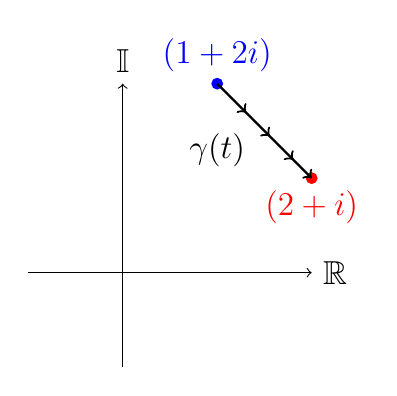
\begin{tikzpicture}
    % Your TikZ code here
    % Example: Draw axes
    \draw[->] (-1,0) -- (2,0) node[right] {$\mathbb{R}$};
    \draw[->] (0,-1) -- (0,2) node[above] {$\mathbb{I}$};
    \draw[thick, blue, fill=blue!100] (1,2) circle (0.05) node[above] {$(1+2i)$};
    \draw[thick, red, fill=red!100] (2,1) circle (0.05) node[below] {$(2+i)$};
                \draw[<-, decoration={markings, 
        mark=at position 0.25 with {\arrow{<}},
        mark=at position 0.5 with {\arrow{<}},
        mark=at position 0.75 with {\arrow{<}}},
      postaction={decorate}, thick] (2,1) -- (1,2);
      \draw (1,1) node[above] {$\gamma(t)$};
\end{tikzpicture}
\end{center}
\vspace{.5cm} 
\hrule 
\vspace{.5cm}
\subsection*{(b)}
A line from $(0,0)$ to point $(1+\sqrt{3}i)$.

This one is quite simple as we only have to multiply the point by $t$ as the first point $P$ is the origin and that handles moving from the origin to the point $(1+\sqrt{3}i)$ as it moves from $0\leq t\leq1$.
\begin{center}
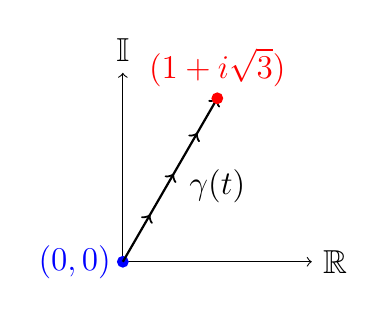
\begin{tikzpicture}
    % Your TikZ code here
    % Example: Draw axes
    \draw[->] (0,0) -- (2,0) node[right] {$\mathbb{R}$};
    \draw[->] (0,0) -- (0,2) node[above] {$\mathbb{I}$};
    \draw[thick, blue, fill=blue!100] (0,0) circle (0.05)node[left] {$(0, 0)$};
                \draw[<-, decoration={markings, 
        mark=at position 0.25 with {\arrow{<}},
        mark=at position 0.5 with {\arrow{<}},
        mark=at position 0.75 with {\arrow{<}}},
      postaction={decorate}, thick] (1, 1.73) -- (0,0);
    \draw[thick, red, fill=red!100] (1, 1.73) circle (0.05) node[above] {$(1+i\sqrt{3})$};
    \draw (1,.5035) node[above] {$\gamma(t)$};
\end{tikzpicture}
\end{center}
\vspace{.5cm} 
\hrule 
\vspace{.5cm}
\subsection*{(c)}
A half-ellipse from point $2$ to $-2$ passing through $i$ centered at the origin.
\begin{align*}
   x & = a \cos{t} = 2\cos{t}\\
  y & = b \sin{t} = \sin{t}\\
  z(t) &= x + iy = 2\cos{t} + \sin{t}
\end{align*}
\begin{center}
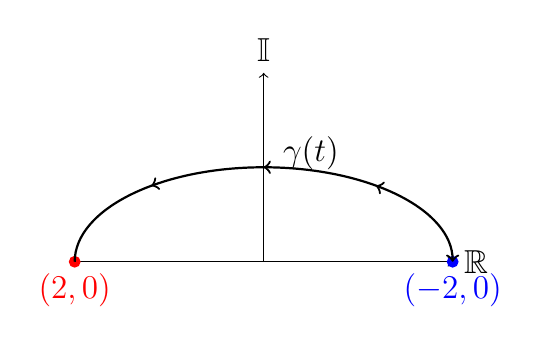
\begin{tikzpicture}
    % Your TikZ code here
    % Example: Draw axes
    \draw[->] (-2,0) -- (2,0) node[right] {$\mathbb{R}$};
    \draw[->] (0,0) -- (0,2) node[above] {$\mathbb{I}$};
    \draw[thick, blue, fill=blue!100] (2,0) circle (0.05)node[below] {$(-2,0)$};
    \draw[thick, red, fill=red!100] (-2,0) circle (0.05) node[below] {$(2,0)$};
                \draw[<-, decoration={markings, 
        mark=at position 0.25 with {\arrow{>}},
        mark=at position 0.5 with {\arrow{>}},
        mark=at position 0.75 with {\arrow{>}}},
      postaction={decorate}, thick] (2, 0) arc (0:180:2 and 1);
      \draw (.5,.85035) node[above] {$\gamma(t)$};
\end{tikzpicture}
\end{center}


\newpage
\section*{Problem 2}
Evaluate the following integrals: 
\begin{enumerate}
\item  $\int_1^2 (\frac{1}{t}-i)^2 dt $
\item $\int_0^{\pi/6} e^{i2t}dt$
\item $\int_0^{\infty} e^{izt}dt$ where $Im(z)>0$ 
\end{enumerate}

\vspace{.5cm} % Space between problems

\hrule
\subsection*{(a)}
\begin{align*}
  \int_1^2 (\frac{1}{t}-i)^2 dt &= \int_1^2 (\frac{1}{t^2} - 2i\frac{1}{t} -i^2) dt \\
  &= \int_1^2\frac{1}{t^2}dt -2i\int_1^2\frac{1}{t}dt + \int_1^2dt \\ 
  &= -\frac{1}{3}\int_1^2-3t^{-2}dt -2i\ln{(t)}|_1^2 + t|_1^2 \\ 
                                &=  -\frac{1}{3}t^{-3}|_1^2 + -2i\ln{(t)}|_1^2 + t|_1^2 \\
                                &= \left(\frac{1}{3}-\frac{1}{3*2^3}\right) - 2i(\ln{(2)}-\ln{(1)}) + 1 \\
                                &= \left(\frac{1}{3}-\frac{1}{3*2^3} + 1 \right) - 2i(\ln{(2)}-0) \\
                                &= \left(\frac{4}{3}-\frac{1}{3*8} \right) - 2i\ln{(2)} \\
                                &= \left(\frac{32}{24}-\frac{1}{24} \right) - 2i\ln{(2)} \\
                                &= \left(\frac{31}{24} \right) - 2i\ln{(2)} 
\end{align*}
\hrule
\subsection*{(b)}
\begin{align*}
  \int_0^{\pi/6} e^{i2t}dt &= \frac{1}{2i}\int_0^{\pi/6} 2ie^{i2t}dt \\
  &= \frac{1}{2i} e^{i2t}|_0^{\pi/6} = -\frac{1}{2}i(e^{i\pi/3} - 1)
\end{align*}
\hrule
\subsection*{(c)}
\begin{align*}
  \int_0^{\infty} e^{izt}dt &=  \frac{1}{iz}e^{izt}|_0^{\infty} = \frac{1}{iz}(e^{iz\infty}-1) \\
  &= \frac{1}{iz}(e^{i(x+iy)\infty}-1) = \frac{1}{iz}(e^{(ix-y)\infty}-1) = \frac{1}{iz}(e^{ix\infty}e^{-y\infty}-1) \\
\end{align*}
$e^{ix\infty}$ oscillates forever and always has a magnitude equal to $1$ no matter the $x$ value. $e^{-y\infty}$ reveals why we need to have the imaginary part grater than $0$. If the imaginary part is greater than 0, we then get exponential decay for the expression involving the negative sign. With this, this eventually dissipates as t approaches infinity.
\begin{align*}
\therefore  \int_0^{\infty} e^{izt}dt &= -\frac{1}{iz}
\end{align*}
\newpage
\section*{Problem 3}
Sketch the oriented curve defined by the following four contours and compute $\int_{C}f(z) dz$ where $f (z) = z-1$:
\begin{enumerate}
\item $C_1$: A semicircle $z=2e^{i\theta}$ for $\theta\in [\pi, 2\pi]$.
\item $C_2$: A full circle $z=2e^{i\theta}$  for $\theta\in [0, 2\pi]$.
\item $C_3$: A line on the real axis from $2$ to $-2$.
\item $C_4 = C_1+C_3$ where $+$ denotes concatenation.
\end{enumerate}

\vspace{.5cm} % Space for work

\hrule
\subsection*{(1)}
\begin{center}
\begin{tikzpicture}
    % Your TikZ code here
    % Example: Draw axes
    \draw[->] (-3,0) -- (3,0) node[right] {$\mathbb{R}$};
    \draw[->] (0,0) -- (0,-3) node[below] {$\mathbb{I}$};
    \draw[thick, blue, fill=blue!100] (2,0) circle (0.05)node[above] {$(2,0)$};
    \draw[thick, red, fill=red!100] (-2,0) circle (0.05) node[above] {$(-2,0)$};
                \draw[>-, decoration={markings, 
        mark=at position 0.25 with {\arrow{>}},
        mark=at position 0.5 with {\arrow{>}},
        mark=at position 0.75 with {\arrow{>}}},
      postaction={decorate}, thick] (-2, 0) arc (0:180:-2 and -2);
      \draw (1,-.85035) node[above] {$\gamma(t)$};
\end{tikzpicture}
\end{center}
\vspace{.5cm} % Space for work
\begin{align*}
f(z) &= z-1 \\
  \gamma(t) &= 2e^{i\pi t}\\
  1 &\leq t \leq 2\\
  t &= 1 \xrightarrow{} e^{i\pi}\\
  t &= 2 \xrightarrow{} e^{i2\pi}\\
  \int_1^{2}f(\gamma(t))\gamma(t)'dt &=  \int_1^{2}(\gamma(t)-1)\gamma(t)'dt\\
  =  \int_1^{2}(2e^{i\pi t}-1)(2i\pi e^{i\pi t})dt &=  2\int_1^{2}(2i\pi e^{i2\pi t})dt- 2\int_1^{2}i\pi e^{i\pi t}dt\\
     &=  2\int_1^{2}(2i\pi e^{i2\pi t})dt- 2\int_1^{2}i\pi e^{i\pi t}dt\\
     &= 2e^{i2\pi t}|_1^2 - 2e^{i\pi t}|_1^2 = 2[(e^{i4\pi}-e^{i2\pi}) - (e^{i2\pi}-e^{i\pi})]\\
     &= 2[(\canceling{1}{e^{i4\pi}}-\canceling{1}{e^{i2\pi}}) - (\canceling{1}{e^{i2\pi}}-\canceling{-1}{e^{i\pi}})] = 2[(1-1) - (1-(-1))] \\
  &= 2(-2) = -4
\end{align*}

\hrule
\newpage
\subsection*{(2)}
The oriented curve is defined as follows:
\begin{center}
\begin{tikzpicture}
    % Your TikZ code here
    % Example: Draw axes
    \draw[->] (-3,0) -- (3,0) node[right] {$\mathbb{R}$};
    \draw[->] (0,-3) -- (0,3) node[above] {$\mathbb{I}$};
    \draw[thick, blue, fill=blue!100] (2,0) circle (0.05)node[below right] {$(2,0)$};
    \draw[thick, red, fill=red!100] (-2,0) circle (0.05) node[below left] {$(-2,0)$};
                \draw[>-, decoration={markings, 
        mark=at position 0.10 with {\arrow{>}},
        mark=at position 0.20 with {\arrow{>}},
        mark=at position 0.30 with {\arrow{>}},
        mark=at position 0.40 with {\arrow{>}},
        mark=at position 0.50 with {\arrow{>}},
        mark=at position 0.60 with {\arrow{>}},
        mark=at position 0.70 with {\arrow{>}},
        mark=at position 0.80 with {\arrow{>}},
        mark=at position 0.90 with {\arrow{>}}},
      postaction={decorate}, thick] (2, 0) arc (0:360:2 and 2);
      \draw (1,.85035) node[above] {$\gamma(t)$};
\end{tikzpicture}
\end{center}
Since we know that the curve here starts and ends at the same point, we know that the overall expression here should evaluate to 0 by the Fundamental Theorem of Calculus. the path $\gamma$
 here has the same starting and ending point, and the function $f(z)$ is continuous everywhere with no discontinuities or issues with branch cuts. The result is then:
\begin{align*}
  f(z) &= z-1 \\
  \gamma(t) &= 2e^{i\pi t}\\
  \int_0^{2}f(\gamma(t))\gamma(t)'dt &=  \int_0^{2}(\gamma(t)-1)\gamma(t)'dt \\
  &=  \int_0^{2}(2e^{i\pi t}-1)(2i\pi e^{i\pi t})dt \\
  &=  \int_0^{2}(2e^{i\pi t}e^{i\pi t}-e^{i\pi t})(2i\pi)dt \\
  &=  (2i\pi)\int_0^{2}(2e^{i2\pi t}-e^{i\pi t})dt \\
  &=  (2i\pi)\left(\frac{2}{i2\pi}e^{i2\pi t}-\frac{1}{i\pi}e^{i\pi t}\right)|_0^{2} \\
  &=  \left(2e^{i2\pi t}-2e^{i\pi t}\right)|_0^{2} \\
  &=  \left(2e^{i4\pi}-2e^{i2\pi}\right) - \left(2e^{0}-2e^{0}\right) \\
  &=  \left(2\cdot 1-2\cdot 1\right) - \left(2-2\right) \\
  &= 0
\end{align*}
\vspace{.5cm} % Space for work

\hrule
\subsection*{(3)}
\begin{center}
\begin{tikzpicture}
    % Your TikZ code here
    % Example: Draw axes
    \draw[->] (-3,0) -- (3,0) node[right] {$\mathbb{R}$};
    \draw[->] (0,0) -- (0,2) node[above] {$\mathbb{I}$};
    \draw[thick, blue, fill=blue!100] (2,0) circle (0.05)node[below right] {$(2,0)$};
    \draw[thick, red, fill=red!100] (-2,0) circle (0.05) node[below left] {$(-2,0)$};
                \draw[->, decoration={markings, 
        mark=at position 0.10 with {\arrow{>}},
        mark=at position 0.20 with {\arrow{>}},
        mark=at position 0.30 with {\arrow{>}},
        mark=at position 0.40 with {\arrow{>}},
        mark=at position 0.50 with {\arrow{>}},
        mark=at position 0.60 with {\arrow{>}},
        mark=at position 0.70 with {\arrow{>}},
        mark=at position 0.80 with {\arrow{>}},
        mark=at position 0.90 with {\arrow{>}}},
      postaction={decorate}, thick] (2, 0) -- (-2,0);
      \draw (1,.25035) node[above] {$\gamma(t)$};
\end{tikzpicture}
\end{center}
\vspace{.5cm} % Space for work
\begin{align*}
  f(z) &= z-1 \\
  \gamma(t) &= z(t) = x(t)+iy(t)\\
  y(t) &= 0 \\
  \x(t) = P + t(Q-P) &= (2,0) + t[(-2,0) - (2,0)] = 2-4t\\
  \gamma(t) &= x(t) = 2-4t\\
  0 &\leq t \leq 1\\
  \int_0^{1}f(\gamma(t))\gamma(t)'dt &=  \int_0^{1}(\gamma(t)-1)\gamma(t)'dt \\
       &=  \int_0^{1}(2-4t-1)(-4)dt =  (-4)\int_0^{1}(1-4t)dt  \\
  &= -4(t-2t^2)|_0^1 = -4[(1-2)-(0)] = -4*(-1) = 4
\end{align*}
\hrule
\newpage
\subsection*{(4)}
\begin{center}
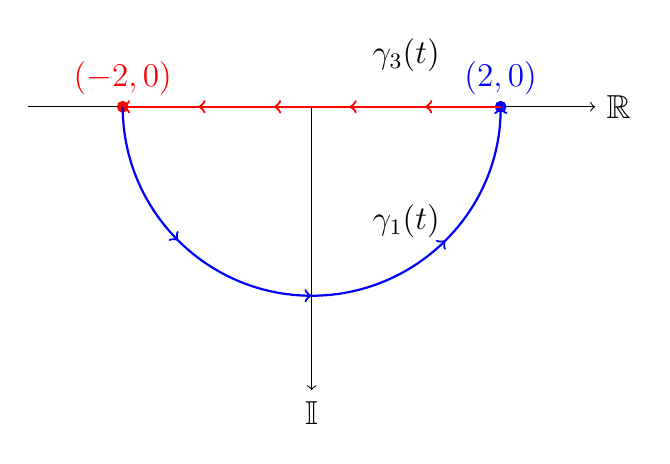
\begin{tikzpicture}
    % Your TikZ code here
    % Example: Draw axes
    \draw[->] (-3,0) -- (3,0) node[right] {$\mathbb{R}$};
    \draw[->] (0,0) -- (0,-3) node[below] {$\mathbb{I}$};
    \draw[thick, blue, fill=blue!100] (2,0) circle (0.05)node[above] {$(2,0)$};
    \draw[thick, red, fill=red!100] (-2,0) circle (0.05) node[above] {$(-2,0)$};
                \draw[->, decoration={markings, 
        mark=at position 0.25 with {\arrow{>}},
        mark=at position 0.5 with {\arrow{>}},
        mark=at position 0.75 with {\arrow{>}}},
      postaction={decorate}, thick, blue] (-2, 0) arc (0:180:-2 and -2);
      \draw (1,-1.5035) node[above] {$\gamma_1(t)$};
                \draw[->, decoration={markings, 
        mark=at position 0.20 with {\arrow{>}},
        mark=at position 0.40 with {\arrow{>}},
        mark=at position 0.60 with {\arrow{>}},
        mark=at position 0.80 with {\arrow{>}}},
      postaction={decorate}, thick, red] (2, 0) -- (-2,0);
      \draw (1,.25035) node[above] {$\gamma_3(t)$};
\end{tikzpicture}
\end{center}
Similar to the case in two, we have a path that that is closed between two points. Since we have evaluated the path previously, we can conclude that this path will also resolve to 0. Taking the answers for 1 and 3 and taking their sum shows this resolves to 0.
\begin{align*}
  \int C_1 + \int C_3 = -4 + 4 = 0
\end{align*}
% Add more problems as needed...

\end{document}

%%% Local Variables:
%%% mode: latex
%%% TeX-master: t
%%% End:
